% Application causality, not unsolicited Data delivery.
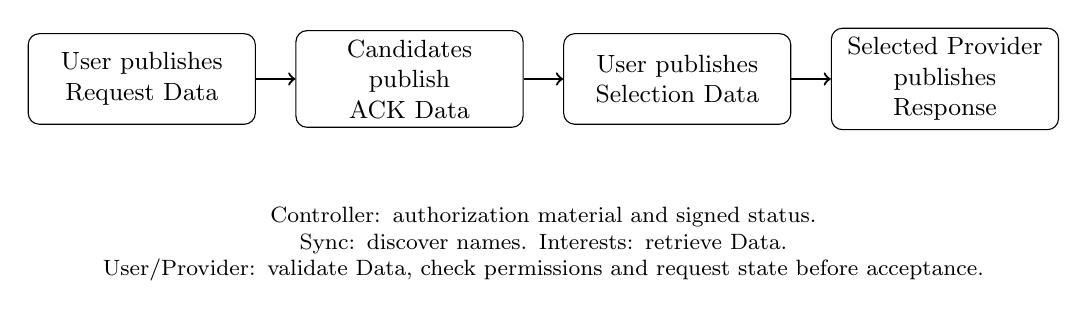
\begin{tikzpicture}[x=1cm,y=1cm,every node/.style={align=center,font=\small}]
\node[draw,rounded corners,text width=2.65cm,minimum height=1.15cm] (r) at (0,0) {User publishes\\Request Data};
\node[draw,rounded corners,text width=2.65cm,minimum height=1.15cm] (a) at (3.4,0) {Candidates publish\\ACK Data};
\node[draw,rounded corners,text width=2.65cm,minimum height=1.15cm] (s) at (6.8,0) {User publishes\\Selection Data};
\node[draw,rounded corners,text width=2.65cm,minimum height=1.15cm] (o) at (10.2,0) {Selected Provider\\publishes Response};
\draw[->,thick] (r)--(a);\draw[->,thick] (a)--(s);\draw[->,thick] (s)--(o);
\node[font=\footnotesize,text width=12cm] at (5.1,-2.1) {Controller: authorization material and signed status.\\Sync: discover names. Interests: retrieve Data.\\User/Provider: validate Data, check permissions and request state before acceptance.};
\end{tikzpicture}
